\documentclass[a4paper, 12pt]{article}
%\usepackage[includleft = 1.5in, right = 1.25in, top = 1in, bottom = 1in]{geometry}
\usepackage{dirtree}
\usepackage{listings}
\usepackage{pdfpages}
\usepackage{fancyhdr}
\usepackage{biblatex}
\usepackage{amsthm}
\usepackage{hyperref}
\usepackage{tcolorbox}


\usepackage{tocloft}
\renewcommand{\cftsecleader}{\cftdotfill{\cftdotsep}}
\renewcommand{\cftsecpagefont}{}% Remove \bfseries from section titles' page in ToC
\usepackage{verbatim}
\usepackage{amsmath}
\usepackage{graphicx}
\usepackage{setspace}
\usepackage{afterpage}

\usepackage{abstract}

\hypersetup{
    colorlinks=true,
    linkcolor=blue,
    filecolor=magenta,      
    urlcolor=blue,
    pdftitle={Overleaf Example},
    pdfpagemode=FullScreen,
  }
  \urlstyle{same}



\renewcommand{\abstractnamefont}{\normalfont\large\bfseries}
%\renewcommand{\baselinestretch}{1.5}
\newcommand\logopath{TU-logo.png}
\newcommand\logofilename{TU-logo}
\newcommand\logoscalefactor{0.7}

\graphicspath{\logoPath}
%\newcommand\myfontsize{\fontsize{14pt}{14pt}\selectfont}
%\setlength{\parindent}{2em}
\renewcommand*\contentsname{Table Of Contents}
\newcommand\myemptypage{
		\null
		\thispagestyle{empty}
		\addtocounter{page}{-1}
		\newpage
}
\lstdefinestyle{mystyle}{frame=tb,
						%language=C++,
						tabsize=3,
						numbersep=5pt}
\lstset{style=mystyle}

% adds bibliography file 
\bibliography{biblio.bib}
\newtheorem{definition}{Definition}

\begin{document}

\begin{titlepage}
\begin{center}
    \textbf{
        \begin{Large}Project Proposal:\\ \end{Large}
      	  \vspace{1\baselineskip} 
      	  \begin{Large}
      	  Cha-insanity:
      	  \vspace{0.3\baselineskip}		
      	  Block Chain Application in Python. 
      	  \end{Large}
    }

    \vspace{0.5\baselineskip}
    {\large Authors:  Prakash Chaulagain, Nishar Arjyal, and Pramish Paudel}\\
   	\large{Roll Numbers: 076BCT045, 076BCT042, 076BCT047} \\
   	\vspace{0.5\baselineskip}
    \centering
      Submitted to the Department of
      Electronics and Computer Engineering
      in Partial Fulfillment of the Requirements for the 2nd Year Data Structures and Algorithms Course\\ 
    at 	\\
    \vspace{0.3\baselineskip}
     \begin{figure}[h!]
    
\includegraphics[width=0.2\linewidth, scale = 0.1]{TU-logo.png}
    \centering
  \end{figure}

    {\large Pulchowk Campus }\\
    {\large IOE, Tribhuwan University}\\
    \vspace{0.3\baselineskip}
    \today\\
  \end{center}
  \vspace{2\baselineskip}
  {
  \raggedright
		Accepted by: \dotfill

  \raggedleft
  \vspace{1\baselineskip}
  Mrs. Bibha Sthapit\\
  Lecturer, Department of Electronics and Computer Engineering\\
	
  }
  \vspace{2\baselineskip}	
	 Date of Submission: \today \\
  	Expected Date of Completion: March, 2022


\end{titlepage}

\myemptypage

\begin{center}
    {\large \textbf{Cha-insanity}}\\
    by 
    {Prakash Chaulagain, Nishar Arjyal, and Pramish Paudel}\\
    \vspace{0.2\baselineskip}
	\begin{spacing}{0.8}
	{Submitted to the Department of Electronics and Computer Engineering \\
	on \today \\ in Partial Fulfillment of the Requirements for the 2nd Year
	Data Structures and Algorithms Course in Computer Engineering}\\
	\end{spacing}    
\end{center}

\begin{abstract}
    Recent times have seen a remarkable surge of decentralized, digital ledger systems that serve as the foundation upon which digital currencies or \emph{cryptocurrencies} operate. Such a digital tool is called \emph{blockchain} which acts as an immutable public ledger and allows transactions to take place in a decentralized manner. Blockchain-based applications have already started making an enormous impact on numerous fields including the financial market, Internet of Things (IoT), elections, digital governance and what not. In this white-paper, we propose one such blockchain application to make a small step forward to opening the door to more financial freedom and a scalable digital economy. We implement our technology in the Python Programming language.
\end{abstract}

\newpage

\newpage
\begin{center}
	\textbf{\myfontsize Acknowledgements}
\end{center} 
\hrule 
\vspace{2\baselineskip}
\par
Our project is the product of excellent supervision and support given 
to us by all of our lab supervisors and our lecturer Mrs. Bibha Sthapit. We are grateful to Mrs Shanti Tamang for her resilience with 
us as our tutor for the last two semesters. We owe everything 
to our supervisors and teachers for their unfaltering support.
\par
Even though times have been tough for the last year and a half, we 
are deeply thankful to the efforts of the entire teaching staff, 
and all the lab supervisors who have not skipped a beat in making sure 
that all of our classes and labs are going on. And some of the 
credit should also go to the administration staff who even though none of 
us has seen in over a year, have quietly done a great job on the sidelines
in making sure that all of the classes are held in a proper manner.

\newpage

\tableofcontents

\newpage 
\pagestyle{fancy}
\fancyhead[C]{Cha-insanity}
\fancyhead[L]{}
\renewcommand{\headrulewidth}{0pt}
\renewcommand{\footrulewidth}{0pt}

\section{Objectives: }
\begin{itemize}
    \item To build a simple block chain application.
    \item To learn the inner workings of existing cryptocurrencies like bitcoin and ethereum.
    \item To become familiar with the literature in cryptography.
    \item To learn Python, a high-level dynamic interpreted programmign language. 
\end{itemize}

\section{Description:}
Of late, blockchain technology has revolutionized the entire field of commerce on the internet. But what exactly is a blockchain? 
We try to answer those questions in this section before we go into the nitty-gritty details of how we propose to implement this advanced technology ourselves. But before we get to answering that, let's set the basics of hashing and cryptography straight. 

\begin{definition}
    \textbf{Hash Function}: A \emph{hash function} is a mathematical function with the following three properties: 
    \begin{itemize}
        \item its input can be any fixed size string,
        \item it produces a fixed-size output,
        \item it is efficiently computable.
    \end{itemize}
\end{definition}

Such a hash function can be used to build any \textbf{\emph{data structure}} notably a hash map and a binary heap that we will come to later in this same section. 

A hash function should have certain properties for it to be valid and safe to use in a professional environment. Here's the properties that we ensure the hash functions we implement will satisfy as a guarantee: 
\begin{itemize}
    \item collision resistance
    \item hiding
    \item puzzle friendliness
\end{itemize}

\begin{definition}
    \textbf{Collision Resistance}: A hash function $H$ is said to be collision resistant if it is infeasible to find two values, $x$ and $y$ such that $x\neq y$ yet $H(x)=H(y)$. 
\end{definition}

\begin{definition}
    \textbf{Hiding}: A hash function is said to be \emph{hiding} if when a secret value r is chosen from a probability distribution that has a high min-entropy, then, given $H(r\parallel x)$, it is infeasible to find x. 
\end{definition}

The intuition behind hiding is that given a commitment, it is infeasible to find a message \emph{msg}. 

\begin{definition}
    \textbf{Puzzle Friendliness}: A hash function $H$ is said to be puzzle friendly if for every possible $n$-bit output value
    $y$, if k is is chosen from a distribution with high-entropy, then it is infeasible to find x such that $H(k\parallel y)=y$ in time significantly less than $2^{n}$.  
\end{definition}

The intuition behind puzzle friendliness is that if someone wants to target hash function to have some particular output value $y$, and if part of the input has been chosen in suitably randomized way, then it is very difficult to find another value that hits the target.

In our implementation, we propose to use the $SHA-256$\footnote{\label{sha256} The standard \href{https://csrc.nist.gov/csrc/media/publications/fips/180/4/final/documents/fips180-4-draft-aug2014.pdf}{SHA256} documentation from NIST} hashing which also happens to be the hashing mechanism used by many popular cryptocurrencies of the sorts of Bitcoin. 

Now, we would like to introduce the reader of this text to the idea of \textbf{\emph{hash pointers}}. 

\textbf{Hash pointers} are just a type of data structure, they are simply pointers to a place where some information is stored together with cryptographic hash or information at some point of time. A regular pointer gives a way to retrieve the information but a hash pointer also allows to verify that the information hasn't been changed. 

Now, we would like to give perhaps the most important definition of our short introduction section : 

\begin{tcolorbox}
    A \textbf{\emph{linked list}} built using hash pointers is the \textbf{\emph{block-chain}}. In a \emph{block-chain}, a block not only tells where the value of the previous block was, but also contains a digest of that value, which allows to verify that the value hasn't changed. 
\end{tcolorbox}

Now, without proof or formally writing a theorem, we make the claim in a casual way that : 

\newpage

\begin{figure}[h!]
    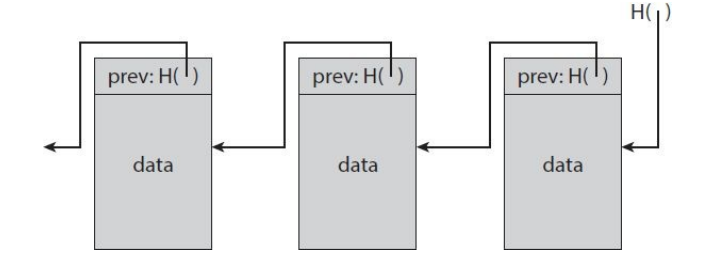
\includegraphics[width=0.7\linewidth, scale = 0.6]{linkedlist.png}
    \centering
    \caption{Block Chain. A block chain is a linked list that is built using hash pointers instead of pointers}
    \label{fig:blockchain}
  \end{figure}




\begin{tcolorbox}
    By remembering the single hash pointer (the head of the list), we can determine a \emph{tamper-evident} hash of the entire list. So, we can build a block chain like this containing as many blocks as we want, going back to some special block at the beginning of the list called \textbf{\emph{genesis block}}.
\end{tcolorbox}

Finally, we explain the idea of \emph{digital signatures} to conclude our introduction off. 
\\~\\
\textbf{A Digital Signature Scheme}:
\\
\\
(sk, pk) := generateKeys(keysize) The generateKeys method takes a key size and generates a key pair. The secret key sk is
kept privately and used to sign messages. pk is the public
verification key that you give to everybody. Anyone with this
key can verify your signature.
\\
\\
sig := sign(sk, message) The sign method takes a message and
a secret key, sk, as input and outputs a signature for message
under sk. 
\\
\\
isValid := verify(pk, message, sig) The verify method takes a
message, a signature, and a public key as input. It returns a
boolean value, isValid, that will be true if sig is a valid
signature for message under public key pk, and false otherwise.

A general cryptocurrency like bitcoin uses a particular digital signature scheme knows as the \emph{
Elliptic Curve Digital Signature Algorithm} (ECDSA). ECDSA is a standard set by the U.S. government. 

\section{Implementation Details}: 

We can create a simple block data structure by doing something like the following pseudocode. 
\begin{lstlisting}[caption=How you could create a Block]
    struct Block 
        index::Int
        timestamp::DateTime
        data::String
        previous_hash::String #length 64 string
            #encoding of hexadecimal no.
        hash::String
        nonce::Int
    end 
\end{lstlisting}

The nonce object represents any random value that appears only once. 

We are yet to do a detailed research of all the more gory details, the algorithms through which we can define transactions in the blockchain. Python has several packages to do encryption and decryption, but this being an academic project means that we are going to try to implement the primitives by ourselves. 

The way currrency is stored and passed between people in decentralized applications is through a wallet model. We think of a wallet as a decentralized bank account. the following general struct block should contain enough information for us to represent such a wallet (in pseudocode):
\begin{lstlisting}[caption=A sufficient wallet structure]
    struct Wallet 
        send::String
        secexp::Int
        private_key::PrivateKey
        public_key::String
    end 
\end{lstlisting}

This wallet basically stores some currency and we don't need someone to verify that our currency is real and valid with the logic of this wallet. Again, we intend to look deeper and do our research for the project to understand further the gory details of the logic of implementation.  

\section{Project Schedule}: 

The project is under development currently.
We intend to share our final project with the class come presentation 
day and it is supposed to be finished by the end of February.
The project should take about three and a half weeks for its completion.

\end{document}

